\section{Approximation to Fisher's wave}\label{sec:S1}

In order to compare the allele frequency and area trajectories of our simulated sweeps to a deterministic model, we modeled an approximation of a positively-selected allele spreading across two-dimensional space as a Fisher wave \citep{fisher_wave_1937}.
The positively-selected allele originates at the center of a 25x25-unit square landscape and spreads in expanding circle whose radius $r$ increases at a velocity $V=M\sqrt{S}$ where $M$ is the rate of per-generation dispersal (similar to the $\sigma$ parameter in the SLiM simulation) and $S$ is the selection coefficient of the allele.
We can therefore define the radius of the circle representing the extent of the sweeping allele at time point $t$ as $r_{edge}(t) = M\sqrt{S}t$ and use this to calculate the area occupied by the allele (Figure \ref{fig:fisher}A).
The width of the wavefront is defined as $W=1/4\sqrt{S}$, thus the spatial extent the fixed allele at time point $t$ can be defined as $r_{fixed}(t) = M\sqrt{S}t - \frac{\sqrt{S}}{4}$.
The circle representing the sweeping wavefront exits the landscape at $R = 12.5$ and completely encompasses the landscape at $R_{max} \approx 17.68$.
If $r_{edge}(t) \leq R$, the area of the sweeping allele is simply $\pi r_{edge}(t)^2$.
If $r_{edge}(t) > R$, the area of the sweeping allele is defined as
$
(\pi - 4\arccos(\frac{R}{r_{edge}}))r_{edge}^2 +
4R{r_{edge}(t)}\sin({\arccos(\frac{R}{r_{edge}(t)})}).
$

To approximate the frequency of the allele, we modeled the sweeping wave in three dimensions as a 
conical frustum - a cone sliced horizontally - with height of 1 along the $z$ axis, an upper radius $r_{fixed}$, and base radius of $r_{edge}$, and calculated its frequency out of the $25 \times 25 \times 1$ volume of the landscape (Figure \ref{fig:fisher}B). If $r_{edge}(t) < R$, then the volume of the conical frustum, $V(t)$, is equal to $\frac{\pi(M\sqrt{S}t)^2}{3} - \frac{\pi(M\sqrt{S}t - \frac{\sqrt{S}}{4})^2}{3}$. If $R \leq r_{edge} \leq R_{max}$ and the base begins to exit the landscape border, then
\begin{multline}
V(t) = (\frac{\pi(M\sqrt{S}t)^2}{3} - \frac{\pi(M\sqrt{S}t - \frac{\sqrt{S}}{4})^2}{3}) - 
(4(\frac{1}{3}(-2R\sqrt{r_{edge}^2 - R^2}) +  \\
(\frac{R^3}{r_{edge}}\ln({\sqrt{r_{edge}^2 - R^2}})
+ r_{edge}) +
(r_{edge}^2\arccos{\frac{R}{r_{edge}}}-\frac{R^3}{r}\ln{R}))),
\end{multline}
removing the volumes of the frustum that are outside the landscape.
Finally, if $r_{edge} > R_{max}$ and the base completely encompasses the landscape,
the volume is calculated as the sum of the volume of a $25 \times 25$ rectangular prism with height $\frac{r_{edge}(t)-R_{max}}{r_{edge}(t)-r_{fixed}(t)}$ and a conical frustum with height $1 - \frac{r_{edge}(t)-R_{max}}{r_{edge}(t)-r_{fixed}(t)}$, base radius $R_{max}$, and upper radius $r_{fixed}(t)$ (after subtracting off volumes of the frustum outside the landscape as described in Equation S1).

Our model recapitulates both the logistic frequency trajectories of a sweep (Figure \ref{fig:fisher}C) and 
the relationship between selection, frequency, and area that we observe in our continuous-space simulations (Figure \ref{fig:fisher}D). We note that the key to the key to the nonlinear relationship between an allele's frequency and area depends on the wavefront where the allele is still segregating; as the strength of selection increases and the width of the wavefront goes to zero the relationship between frequency and area becomes linear.

\begin{figure}[htp]
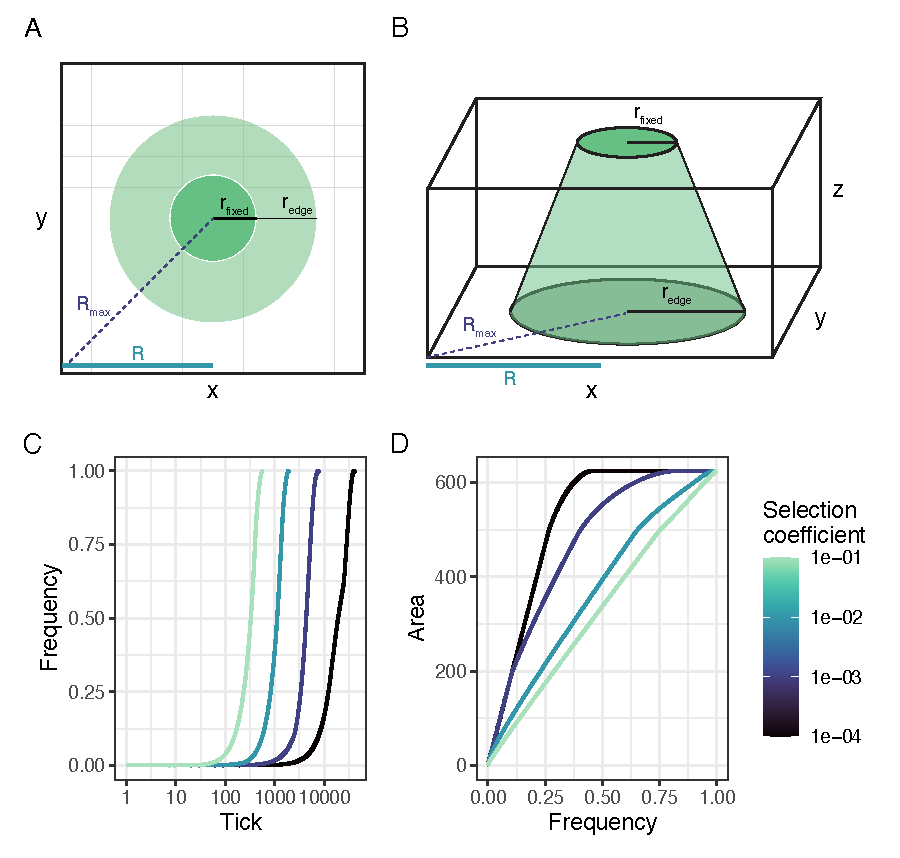
\includegraphics[width=\linewidth]{figures/supplement-fisherwave.pdf}
\centering
\caption{Approximation of a positively-selected allele spreading according to a Fisher wave across two-dimensional space.
(A) Top-down view of the extent of the sweeping allele ($r_{edge}$)
and the extent of the allele's fixation ($r_{fixed}$).
(B) Side view of the method used to approximate the frequency of the sweeping allele as the volume of the conical frustum defined by $r_{edge}$ and $r_{fixed}$ out of the volume of the landscape defined by $x$, $y$, and $z$.
(C) Frequency of the positively-selected allele. 
(D) Joint distribution between frequency and area of the positively selected allele.
In both plots, lines are colored by selection coefficient ($S$).}
\label{fig:fisher}
\end{figure}

\begin{figure}[htp]
\includegraphics[width=\linewidth]{figures/supplement-power_analysis_by_frequency.pdf}
\centering
\caption{Probability of detecting a sweeping allele as a spatial outlier over the course of a sweep across dispersal distances (x axis) and cutoff percentiles (y axis). Lines are colored by selection coefficient.}
\label{fig:poweranalysisoutlierprop}
\end{figure}

\begin{figure}[htp]
\includegraphics[width=\linewidth]{figures/supplement-inversionjdist.pdf}
\centering
\caption{Joint frequency-area distribution for \textit{An. gambiae} SNPs within the 2La (A), 2Rb (B), and 2Rc (C) inversions.
SNPs are colored according to their SNPEff annotation; black lines represent the 10th percentile cutoff.}
\label{fig:inversionjdist}
\end{figure}

%\comment{figure: admixture results}